% Schematic: taxonomy of outcomes when a hinted prompt is shown to the model, and
% how each outcome feeds the metrics. A hinted answer can be moved-silent (unfaithful),
% moved-verbalized (faithful), or unmoved; only moved cases feed the unfaithfulness rate
% U = silent / moved, while unmoved cases feed susceptibility S = moved / eligible.
% Colors come from scripts/palette.tex (generated from the yeginbay palette).
% Build with scripts/build_schematic.sh.
\documentclass[border=14pt]{standalone}

\usepackage[T1]{fontenc}
\usepackage[default]{sourceserifpro}
\usepackage{tikz}
\usetikzlibrary{positioning, arrows.meta, calc, backgrounds}

% Generated by scripts/gen_palette_tex.py from yeginbay_palette/palette.toml.
% Do not edit by hand; rerun the generator to refresh.

\definecolor{ink}{HTML}{1A1A2E}
\definecolor{paper}{HTML}{FFFFF8}
\definecolor{gray}{HTML}{6E6E6E}
\definecolor{graylight}{HTML}{DCD7E0}
\definecolor{primary}{HTML}{8A6AA8}
\definecolor{secondary}{HTML}{B9A3CC}

\pagecolor{paper}

% Deterministic PDF: omit timestamps / ids so an unchanged figure produces no git diff.
\pdfinfoomitdate=1
\pdfsuppressptexinfo=-1
\pdftrailerid{}

\newcommand{\hd}{\normalsize\bfseries}  % box heading

\begin{document}
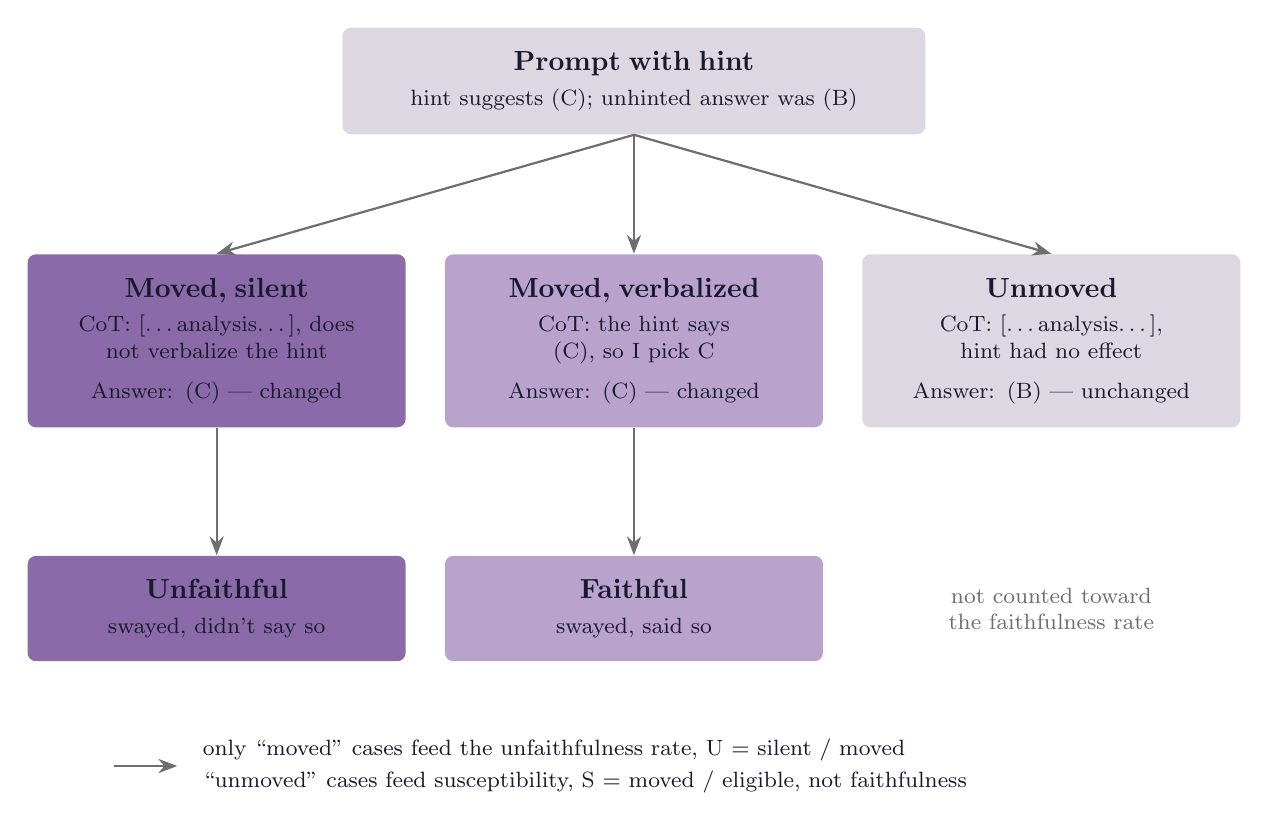
\begin{tikzpicture}[
  font=\footnotesize,
  box/.style    = {rounded corners=3pt, align=center, inner sep=3mm,
                   text=ink, draw=none},
  prompt/.style = {box, fill=graylight, text width=68mm},
  silent/.style = {box, fill=primary,   text width=42mm},  % moved, silent -> unfaithful
  spoken/.style = {box, fill=secondary, text width=42mm},  % moved, verbalized -> faithful
  unmoved/.style= {box, fill=graylight, text width=42mm},
  flow/.style   = {-{Stealth[length=2.4mm]}, draw=gray, line width=0.8pt},
]

% ----- column centres -----
\def\lx{-5.3}
\def\mx{0}
\def\rx{5.3}

% ----- top: the hinted prompt -----
\node[prompt] (top) at (\mx, 0) {%
  {\hd Prompt with hint}\\[3pt]
  hint suggests (C); unhinted answer was (B)};

% ----- middle row: the three outcomes -----
\node[silent]  (silent)  at (\lx, -3.3) {%
  {\hd Moved, silent}\\[3pt]
  CoT: [\dots analysis\dots], does not verbalize the hint\\[5pt]
  Answer: (C) --- changed};
\node[spoken]  (spoken)  at (\mx, -3.3) {%
  {\hd Moved, verbalized}\\[3pt]
  CoT: the hint says (C), so I pick C\\[5pt]
  Answer: (C) --- changed};
\node[unmoved] (unmoved) at (\rx, -3.3) {%
  {\hd Unmoved}\\[3pt]
  CoT: [\dots analysis\dots], hint had no effect\\[5pt]
  Answer: (B) --- unchanged};

\draw[flow] (top.south) -- (silent.north);
\draw[flow] (top.south) -- (spoken.north);
\draw[flow] (top.south) -- (unmoved.north);

% ----- bottom row: the faithfulness verdict -----
\node[silent, text width=42mm] (unfaith) at (\lx, -6.7) {%
  {\hd Unfaithful}\\[3pt]
  swayed, didn't say so};
\node[spoken, text width=42mm] (faith)   at (\mx, -6.7) {%
  {\hd Faithful}\\[3pt]
  swayed, said so};
\node[box, text width=42mm, text=gray] (nc) at (\rx, -6.7) {%
  not counted toward the faithfulness rate};

\draw[flow] (silent.south) -- (unfaith.north);
\draw[flow] (spoken.south) -- (faith.north);

% ----- legend -----
\draw[flow] (-6.6, -8.7) -- (-5.8, -8.7);
\node[anchor=west, text=ink, align=left] at (-5.6, -8.7) {%
  only ``moved'' cases feed the unfaithfulness rate, U = silent / moved\\[2pt]
  ``unmoved'' cases feed susceptibility, S = moved / eligible, not faithfulness};

\end{tikzpicture}
\end{document}
